

\documentclass{beamer}
\usepackage{HECbeamer}
% \usepackage{pgfpages}
% \pgfpagesuselayout{4 on 1}[letterpaper, landscape, border shrink=5mm]
\title[\color{white}{MATH 60604A \S~4b - Logistic regression}]{\texorpdfstring{MATH 60604A \\Statistical modelling \\ \S~4b - Logistic regression}{MATH 60604A \\Statistical modelling \\ \S~4b - Logistic regression}}
\author{}
\institute{HEC Montréal\\
Department of Decision Sciences}
\date{} 

\begin{document}
\frame{\titlepage}

\begin{frame}[fragile]
\frametitle{Generalized linear model for binary variables}
% 
% Generalized linear models are parametrized in terms of \emph{function} of the mean $g(\mu_i)$ in terms of the linear combination $\eta_i$:
% 
% \begin{align*}
% g\left\{\E{Y_i \mid \mathbf{X}_i}\right\}&=\beta_0+ \beta_1 \mathrm{X}_{i1} + \cdots + \beta_p \mathrm{X}_{ip}
% \intertext{or equivalently}
% \E{Y_i \mid \mathbf{X}_i}&=g^{-1} \left( \beta_0+ \beta_1 \mathrm{X}_{i1} + \cdots + \beta_p \mathrm{X}_{ip} \right).
% \end{align*}
\bi
\item In the case of a binary response variable, assume $Y_i $ follows a Bernoulli distribution with parameter $\pi_i$, $Y_i\sim \mathsf{Bin}(\pi_i) $, where 
\[\pi_i= \P{Y_i=1 \mid \mathbf{X}_i}=\E{Y_i \mid \mathbf{X}_i}.\]

% \item Thus, logistic regression allows to model the mean $\mu_i = \E{Y_i\mid \mathbf{X}_i}$ in terms of the explanatory variables via an appropriate link function $g$
% \begin{align*}
% g\left(\mu_i\right) = g\left(\pi_i\right)=\beta_0+ \beta_1 \mathrm{X}_{i1} + \cdots + \beta_p \mathrm{X}_{ip}
% \end{align*}
% \item The logistic regression model makes the link between $\pi_i$ and the variables $\mathbf{X}_i$
% \ei
% \end{frame}



%\begin{align*}
%\ln\left(\frac{\mu_i}{1-\mu_i}\right)=\ln\left(\frac{\P{Y_i=1}}{1-\P{Y_i=1}}\right)=\beta_0+ \beta_1 \mathrm{X}_{i1}+\ldots+\beta_p \mathrm{X}_{ip}
%\end{align*}
%\ei
%\end{frame}
% \begin{frame}[fragile]
% \frametitle{Logistic regression}
% \bi
\item An appropriate link function for binary responses is the \alert{logit} function
\begin{align*}
g(z)\coloneqq\logit(z)=\ln\left(\frac{z}{1-z}\right).
\end{align*}
\item The \textbf{logistic regression model} is 
\begin{align*}
g(\pi_i) = \ln\left(\frac{\pi_i}{1-\pi_i}\right)= \eta_i \coloneqq\beta_0+ \beta_1 \mathrm{X}_{i1}+\cdots+\beta_p \mathrm{X}_{ip}.
\end{align*}

\item The logit function $g$ is the \textbf{quantile function of the logistic distribution} and \alert{links} $\E{Y_i\mid \mathbf{X}_i}=\pi_i(\mathbf{X}_i)$ and $\eta_i$.
\ei
\end{frame}


% 
% \begin{frame}[fragile]
% \frametitle{Definition of odds }
% \bi
% \item The following table gives several examples of probabilities $\P{Y=1}$ and their corresponding odds:
%     
% 
% \begin{center}
% \begin{tabular}{c c}
% \toprule
% $\P{Y=1}$ & Odds \\ \midrule
% $0.1$ & $0.11$ \\
% $0.2$ & $0.25$ \\
% $0.3$ & $0.43$ \\
% $0.4$ & $0.67$ \\
% $0.5$ & $1$ \\
% $0.6$ & $1.5$ \\ 
% $0.7$ & $2.33$ \\
% $0.8$ & $4$ \\
% $0.9$ & $9$ \\ \bottomrule
% \end{tabular}
% \end{center}
% %\begin{center}
% %\includegraphics[scale=0.5]{Figures/log21.pdf}
% %\end{center}
% \ei
% \end{frame}
% \begin{frame}{Range of the logit transform}
% \bi 
% \item In the case of a binary response, the mean is
% \begin{align*}
% \mu_i = \E{Y_i \mid\mathbf{X}}= \P{Y_i=1\mid \mathbf{X}_i}=\pi_i,
% \end{align*}
% and a probability must lie in $[0, 1]$.
% \item We cannot use an identity link as for normal response, because 
%  \begin{align*}
% \eta_i =\beta_0+ \beta_1 \mathrm{X}_{i1}+\ldots+\beta_p \mathrm{X}_{ip}
% \end{align*}
% can take any value in $(-\infty, \infty)$.
% \item By using the logit link function, we ensure that $\pi_i$ always falls in the $[0, 1]$ interval, since $\logit(\pi) \in (-\infty, \infty)$ if $\pi \in (0,1)$.
% % \begin{align*}
% % \underbrace{\ln\left(\frac{\pi_i}{1-\pi_i}\right)}_{\in (-\infty, +\infty)}=\underbrace{\beta_0+ \beta_1 \mathrm{X}_{i1}+\ldots+\beta_p \mathrm{X}_{ip}}_{\in (-\infty, +\infty)}
% % \end{align*}
% \item Using the logit link function also makes the form of the underlying likelihood function more amenable to maximization (canonical link function).
% \ei
% 
% \end{frame}




\begin{frame}[fragile]
\frametitle{Logistic regression: logit function}
\bi
\item The logistic model is
\begin{align*}
\eta_i=\ln\left(\frac{\pi_i}{1-\pi_i}\right)=\beta_0+ \beta_1 \mathrm{X}_{i1} + \cdots + \beta_p \mathrm{X}_{ip}.
\end{align*}
\item This model can also be written on the mean scale by using the \alert{inverse-logit} (expit) function, 
\begin{align*}
\E{Y_i \mid \mathbf{X}_i}=\pi_i=\frac{\exp(\beta_0+ \beta_1  \mathrm{X}_{i1} + \cdots + \beta_p \mathrm{X}_{ip})}{1+\exp(\beta_0+ \beta_1  \mathrm{X}_{i1} + \cdots + \beta_p \mathrm{X}_{ip})}.
\end{align*}
\item We have an expression for the mean $\pi_i=\E{Y_i\mid \mathbf{X}_i}$ as a function of the explanatory variables $\mathbf{X}_i$, but\ldots
\bi
 
\item what does this function look like?
\item what does this tell us about the relationship between $\pi_i$ and $\eta_i$ (and thus $\mathbf{X}_i$)?
\ei
\ei
\end{frame}

\begin{frame}[fragile]
\frametitle{Logistic distribution function}



\begin{center}
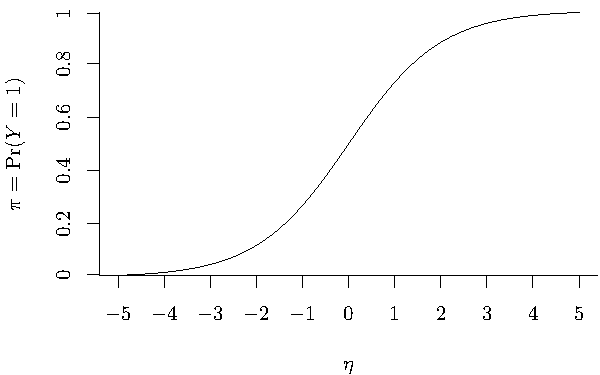
\includegraphics[width = 0.7\linewidth]{img/c4/08-glm-logisticcdf}
\end{center}
\bi
\item Notice $\pi$ is an \textbf{increasing function} of $\eta=\beta_0 + \sum_{j=1}^p \beta_j \mathrm{X}_{j}$.
{\small \bi 
\item If $\beta_j$ is positive and $\mathrm{X}_{j}$ increases, $\P{Y=1}$ also increases.  
\item If $\beta_j$ is negative and $\mathrm{X}_{j}$ increases, $\P{Y=1}$ decreases. 
\ei
}
\item We also see that the relationship between $\P{Y=1}$ and $\eta$ (and thus each $\mathrm{X}_{j}$) is \alert{non-linear}.
\ei
\end{frame}
% 
% \begin{frame}[fragile]
% \frametitle{Logistic regression: logit function}
% \bi
% \item Here's another example with $\beta_0=1$ and $\beta_1=-2$. The graph shows $\P{Y=1}$ as a function of $\mathrm{X}$
% 
% 
% \begin{center}
% \includegraphics[scale=0.2]{Figures/log9.pdf}
% \end{center}
% \item When $\mathrm{X}$ increases, the probability that $Y=1$ decreases because the slope coefficient $\beta_1$ is negative.
% \ei
% \end{frame}
% 
% \begin{frame}[fragile]
% \frametitle{Logistic regression: coefficient interpretation}
% \begin{tcolorbox}[colback=white, colframe=hecblue, title=General interpretation]
% \bi
% \item If $\beta_j$ is positive, the higher the value of $\beta_j$, the higher the probability that $Y=1$ \alert{increases} with the value of $\mathrm{X}_j$.
% \item If $\beta_j$ is negative, the higher the value of $|\beta_j|$, the more the probability that $Y=1$ decreases with the value of $\mathrm{X}_j$.
% \ei
% \end{tcolorbox}
% % \begin{align*}
% % \ln\left(\frac{\pi_i}{1-\pi_i}\right)=\beta_0+ \beta_1 \mathrm{X}_{i}
% % \end{align*}
% 
% \end{frame}

\begin{frame}[fragile]
\frametitle{Parameter interpretations in terms of odds}
\bi
\item Quantifying the effect sizes in logistic regression is not easy because it's a nonlinear model.
\item The coefficients can be interpreted in terms of \alert{odds} and \alert{odds ratios}.
\item Let $\pi=\P{Y=1\mid \mathrm{X}_1, \ldots, \mathrm{X}_p}$, the logistic regression model is 
\begin{align*}
\ln\left(\frac{\pi}{1-\pi}\right)=\beta_0+ \beta_1 \mathrm{X}_1 + \cdots + \beta_p\mathrm{X}_p.
\end{align*}
\item By exponentiating both sides, we obtain 
\begin{align*}
\mathrm{odds}(Y\mid \mathbf{X}) = \frac{\pi(\mathbf{X})}{1-\pi(\mathbf{X})}=\exp(\beta_0+ \beta_1 \mathrm{X}_1 + \cdots + \beta_p\mathrm{X}_p),
\end{align*}
where $\pi(\mathbf{X})/\{1-\pi(\mathbf{X})\}$ are the odds of $\P{Y=1 \mid \mathbf{X}}$ relative to $\P{Y=0 \mid\mathbf{X}}$.
\ei
\end{frame}



\begin{frame}[fragile]
\frametitle{Odds}
\bi
\item The logit function corresponds to modelling the \textbf{log-odds}.

\item The odds for binary $Y$ are the quotient 
\begin{align*}
 \mathrm{odds}(\pi) = \frac{\pi}{1-\pi} = \frac{\P{Y=1}}{\P{Y=0}}.
\end{align*}

\item For example, an odds of $4$ means that the probability that $Y=1$ is four times higher than the probability that $Y=0$. 
\item An odds of $0.25$ means the probability that $Y=1$ is only a quarter times the probability that $Y=0$, or equivalently, the probability that $Y=0$ is four times higher than the probability that $Y=1$.
\ei

\begin{tabular}{lccccccccc}
\toprule
 $\P{Y=1}$& $0.1$ & $0.2$ & $0.3$ & $0.4$ & $0.5$ & $0.6$& $0.7$ & $ 0.8$& $0.9$\\
 Odds & $0.11$ & $0.25$ & $0.43$ & $0.67$ & $1$ &$1.5$ & $2.33$ & $4$ & $9$\\
 Odds (frac.) & $\frac{1}{9}$ & $\frac{1}{4}$
 & $\frac{3}{7}$ & $\frac{2}{3}$ & $1$ & $\frac{3}{2}$ & $\frac{7}{3}$ & $4$ & $9$\\
 \bottomrule
 
\end{tabular}

% \item If we were to use the identity link (as in linear regression) we would have
% \small{
% \begin{align*}
% \mu_i=\E{Y_i\mid \mathbf{X}_i} = \beta_0+ \beta_1 \mathrm{X}_{i1}+\ldots+\beta_p \mathrm{X}_{ip}
% \end{align*}}
% \item The problem is that the linear combination 
% \begin{align*}
% \eta_i =\beta_0+ \beta_1 \mathrm{X}_{i1}+\ldots+\beta_p \mathrm{X}_{ip}
% \end{align*}
% can theoretically take on any value in $(-\infty, \infty)$, which in turn would imply that the mean $\mu_i$ can take on any value in $(-\infty, \infty)$

% \ei 
\end{frame}
\begin{frame}[fragile]
\frametitle{Interpretation of the intercept in terms of the odds}
\bi
\item When $\mathrm{X}_1=\cdots = \mathrm{X}_p=0$, it is clear that 
\begin{align*}
\mathrm{odds}(Y\mid \mathbf{X}=\bs{0}_p) = \exp(\beta_0)
\end{align*}
and 
\begin{align*}
\P{Y=1\mid \mathrm{X}_1=0, \ldots \mathrm{X}_p=0} = \frac{\exp({\beta_0})}{1+\exp({\beta_0})}
\end{align*}
which represents the probability that $Y=1$ when $\mathbf{X}=\bs{0}_p$.
\item As for linear regression, $\mathrm{X}_1=\cdots =\mathrm{X}_p=0$ might not be physically possible, in which case there is no sensible interpretation for $\beta_0$.
\ei
\end{frame}

\begin{frame}[fragile]
\frametitle{Parameter interpretation in terms of the odds ratio}
Consider for simplicity a logistic model of the form 
\[\logit(\pi) = \beta_0 + \beta_1x.\]
The factor $\exp(\beta_1)$ is the change in odds when $\mathrm{X}$ increases by one unit,
\begin{align*}
\mathrm{odds}(Y \mid  \mathrm{X}=x+1) = \exp(\beta_1) \times \mathrm{odds}(Y \mid  \mathrm{X}=x).
\end{align*}
\bi
\item If $\beta_1=0$ then the odds ratio is unity,
\bi
 \item[] meaning that the variable $\mathrm{X}$ is not associated with the odds of $Y$
\ei
\item If $\beta_1$ is positive, then the odds ratio $\exp(\beta_1)$ is larger than one,
\bi
 
\item[] meaning that, as $\mathrm{X}$ increases, the odds of $Y$ increases.
\ei
\item If $\beta_1$ is negative, the odds ratio $\exp(\beta_1)$ is smaller than one,
\bi
 
\item[] meaning that, as $\mathrm{X}$ increases, the odds of $Y$ decreases.
\ei
\ei 

\footnotesize{Note that, when there are several explanatory variables in the model, the interpretation of $\beta_1$ is \alert{when all other variables in the model are held constant.}

}

\end{frame}
\begin{frame}[fragile]
\frametitle{Interpretation of $\beta_k$ in terms of odds ratio}

For the logistic model,  the \alert{odds ratio} when $\mathrm{X}_k=x_k+1$ versus $\mathrm{X}_k=x_k$ when $\mathrm{X}_j=x_j$ $(j=1, \ldots, p, j \neq k)$ is
{\small
\begin{align*}
\frac{\mathrm{odds}(Y \mid  \mathrm{X}_k=x_k+1, \mathrm{X}_j=x_j, j\neq k)}{\mathrm{odds}(Y \mid \mathrm{X}_k=x_k, \mathrm{X}_j=x_j, j \neq k)}&=\frac{\exp\left(\beta_0+ \sum_{j=1}^p\beta_j x_j + \beta_k \right)}{\exp\left(\beta_0+ \sum_{j=1}^p\beta_j x_j \right)}\\
&= \exp(\beta_k).
\end{align*}
}

When $\mathrm{X}_k$ increases by one unit \textbf{and all the other covariates are held constant}, the odds of $Y$ changes by a factor $\exp(\beta_k)$.
\bi \item The odds increase if $\exp(\beta_k) >1$, i.e., if $\beta_k>0$.
\item The odds decrease if $\exp(\beta_k) < 1$, i.e., if $\beta_k<0$.
\ei
The effect of $\beta_k$ is larger when $\pi$ is near $0.5$ than near endpoints of $(0, 1)$.
\end{frame}
\end{document}
